% Options for packages loaded elsewhere
\PassOptionsToPackage{unicode}{hyperref}
\PassOptionsToPackage{hyphens}{url}
\PassOptionsToPackage{dvipsnames,svgnames,x11names}{xcolor}
%
\documentclass[
]{interact}

\usepackage{amsmath,amssymb}
\usepackage{lmodern}
\usepackage{iftex}
\ifPDFTeX
  \usepackage[T1]{fontenc}
  \usepackage[utf8]{inputenc}
  \usepackage{textcomp} % provide euro and other symbols
\else % if luatex or xetex
  \usepackage{unicode-math}
  \defaultfontfeatures{Scale=MatchLowercase}
  \defaultfontfeatures[\rmfamily]{Ligatures=TeX,Scale=1}
  \setmainfont[]{Roboto}
  \setsansfont[]{Roboto}
\fi
% Use upquote if available, for straight quotes in verbatim environments
\IfFileExists{upquote.sty}{\usepackage{upquote}}{}
\IfFileExists{microtype.sty}{% use microtype if available
  \usepackage[]{microtype}
  \UseMicrotypeSet[protrusion]{basicmath} % disable protrusion for tt fonts
}{}
\makeatletter
\@ifundefined{KOMAClassName}{% if non-KOMA class
  \IfFileExists{parskip.sty}{%
    \usepackage{parskip}
  }{% else
    \setlength{\parindent}{0pt}
    \setlength{\parskip}{6pt plus 2pt minus 1pt}}
}{% if KOMA class
  \KOMAoptions{parskip=half}}
\makeatother
\usepackage{xcolor}
\setlength{\emergencystretch}{3em} % prevent overfull lines
\setcounter{secnumdepth}{5}
% Make \paragraph and \subparagraph free-standing
\ifx\paragraph\undefined\else
  \let\oldparagraph\paragraph
  \renewcommand{\paragraph}[1]{\oldparagraph{#1}\mbox{}}
\fi
\ifx\subparagraph\undefined\else
  \let\oldsubparagraph\subparagraph
  \renewcommand{\subparagraph}[1]{\oldsubparagraph{#1}\mbox{}}
\fi


\providecommand{\tightlist}{%
  \setlength{\itemsep}{0pt}\setlength{\parskip}{0pt}}\usepackage{longtable,booktabs,array}
\usepackage{calc} % for calculating minipage widths
% Correct order of tables after \paragraph or \subparagraph
\usepackage{etoolbox}
\makeatletter
\patchcmd\longtable{\par}{\if@noskipsec\mbox{}\fi\par}{}{}
\makeatother
% Allow footnotes in longtable head/foot
\IfFileExists{footnotehyper.sty}{\usepackage{footnotehyper}}{\usepackage{footnote}}
\makesavenoteenv{longtable}
\usepackage{graphicx}
\makeatletter
\def\maxwidth{\ifdim\Gin@nat@width>\linewidth\linewidth\else\Gin@nat@width\fi}
\def\maxheight{\ifdim\Gin@nat@height>\textheight\textheight\else\Gin@nat@height\fi}
\makeatother
% Scale images if necessary, so that they will not overflow the page
% margins by default, and it is still possible to overwrite the defaults
% using explicit options in \includegraphics[width, height, ...]{}
\setkeys{Gin}{width=\maxwidth,height=\maxheight,keepaspectratio}
% Set default figure placement to htbp
\makeatletter
\def\fps@figure{htbp}
\makeatother
\newlength{\cslhangindent}
\setlength{\cslhangindent}{1.5em}
\newlength{\csllabelwidth}
\setlength{\csllabelwidth}{3em}
\newlength{\cslentryspacingunit} % times entry-spacing
\setlength{\cslentryspacingunit}{\parskip}
\newenvironment{CSLReferences}[2] % #1 hanging-ident, #2 entry spacing
 {% don't indent paragraphs
  \setlength{\parindent}{0pt}
  % turn on hanging indent if param 1 is 1
  \ifodd #1
  \let\oldpar\par
  \def\par{\hangindent=\cslhangindent\oldpar}
  \fi
  % set entry spacing
  \setlength{\parskip}{#2\cslentryspacingunit}
 }%
 {}
\usepackage{calc}
\newcommand{\CSLBlock}[1]{#1\hfill\break}
\newcommand{\CSLLeftMargin}[1]{\parbox[t]{\csllabelwidth}{#1}}
\newcommand{\CSLRightInline}[1]{\parbox[t]{\linewidth - \csllabelwidth}{#1}\break}
\newcommand{\CSLIndent}[1]{\hspace{\cslhangindent}#1}

\usepackage{soul}
\usepackage{xcolor}
\definecolor{highlighter}{HTML}{FFFF66}
\sethlcolor{highlighter}
\newcommand{\rev}[1]{\hl{#1}}
%\newcommand{\rev}[1]{#1}
\usepackage{booktabs}
\usepackage{longtable}
\usepackage{array}
\usepackage{multirow}
\usepackage{wrapfig}
\usepackage{float}
\usepackage{colortbl}
\usepackage{pdflscape}
\usepackage{tabu}
\usepackage{threeparttable}
\usepackage{threeparttablex}
\usepackage[normalem]{ulem}
\usepackage{makecell}
\usepackage{xcolor}
\usepackage{orcidlink}
\makeatletter
\makeatother
\makeatletter
\makeatother
\makeatletter
\@ifpackageloaded{caption}{}{\usepackage{caption}}
\AtBeginDocument{%
\ifdefined\contentsname
  \renewcommand*\contentsname{Table of contents}
\else
  \newcommand\contentsname{Table of contents}
\fi
\ifdefined\listfigurename
  \renewcommand*\listfigurename{List of Figures}
\else
  \newcommand\listfigurename{List of Figures}
\fi
\ifdefined\listtablename
  \renewcommand*\listtablename{List of Tables}
\else
  \newcommand\listtablename{List of Tables}
\fi
\ifdefined\figurename
  \renewcommand*\figurename{Figure}
\else
  \newcommand\figurename{Figure}
\fi
\ifdefined\tablename
  \renewcommand*\tablename{Table}
\else
  \newcommand\tablename{Table}
\fi
}
\@ifpackageloaded{float}{}{\usepackage{float}}
\floatstyle{ruled}
\@ifundefined{c@chapter}{\newfloat{codelisting}{h}{lop}}{\newfloat{codelisting}{h}{lop}[chapter]}
\floatname{codelisting}{Listing}
\newcommand*\listoflistings{\listof{codelisting}{List of Listings}}
\makeatother
\makeatletter
\@ifpackageloaded{caption}{}{\usepackage{caption}}
\@ifpackageloaded{subcaption}{}{\usepackage{subcaption}}
\makeatother
\makeatletter
\@ifpackageloaded{tcolorbox}{}{\usepackage[many]{tcolorbox}}
\makeatother
\makeatletter
\@ifundefined{shadecolor}{\definecolor{shadecolor}{rgb}{.97, .97, .97}}
\makeatother
\makeatletter
\makeatother
\ifLuaTeX
  \usepackage{selnolig}  % disable illegal ligatures
\fi
\IfFileExists{bookmark.sty}{\usepackage{bookmark}}{\usepackage{hyperref}}
\IfFileExists{xurl.sty}{\usepackage{xurl}}{} % add URL line breaks if available
\urlstyle{same} % disable monospaced font for URLs
\hypersetup{
  pdftitle={Choropleth Maps Can Convey Magnitude Through the Range of the Accompanying Color Legend},
  pdfauthor={Duncan Bradley; Boshuo Zhang; Caroline Jay; Andrew J. Stewart},
  pdfkeywords={visualisation, cognition, colour, framing effect},
  colorlinks=true,
  linkcolor={blue},
  filecolor={Maroon},
  citecolor={Blue},
  urlcolor={Blue},
  pdfcreator={LaTeX via pandoc}}

\title{Choropleth Maps Can Convey Magnitude Through the Range of the
Accompanying Color Legend}
\author{Duncan
Bradley$\textsuperscript{1}$~\orcidlink{0000-0001-7328-8779}, Boshuo
Zhang$\textsuperscript{2}$~\orcidlink{0000-0003-0477-9122}, Caroline
Jay$\textsuperscript{2}$~\orcidlink{0000-0002-6080-1382}, Andrew J.
Stewart$\textsuperscript{2}$~\orcidlink{0000-0002-9795-4104}}

\thanks{CONTACT: Duncan
Bradley. Email: \href{mailto:duncan.bradley@manchester.ac.uk}{\nolinkurl{duncan.bradley@manchester.ac.uk}}. }
\begin{document}
\maketitle
\textsuperscript{1} Division of Psychology, Communication, and Human
Neuroscience, The University of
Manchester, Manchester, UK\\ \textsuperscript{2} Department of Computer
Science, The University of Manchester, Manchester, UK
\begin{abstract}
Data visualization software provides the ability to create highly
customizable choropleth maps. This presents an abundance of design
choices. The color legend, one particular aspect of choropleth map
design, has the potential to effectively convey data points' magnitudes
(how large or small they are). Color legends present the mapping between
a specific range of colors and a specific range of numerical values. In
this experiment, we demonstrate that manipulating this range affects
interpretations of the magnitude of plotted values. Participants (N =
100) judged the urgency of addressing pollution levels as greater when
the color legend's upper bound was equal to the maximum plotted value,
compared to when it was significantly larger than the maximum plotted
value. This provides insight into the cognitive processing of plotted
data in choropleth maps that are designed to promote inferences about
overall magnitude.
\end{abstract}
\begin{keywords}
\def\sep{;\ }
visualisation\sep cognition\sep colour\sep 
framing effect
\end{keywords}
\ifdefined\Shaded\renewenvironment{Shaded}{\begin{tcolorbox}[borderline west={3pt}{0pt}{shadecolor}, breakable, enhanced, sharp corners, interior hidden, boxrule=0pt, frame hidden]}{\end{tcolorbox}}\fi

\hypertarget{sec-intro}{%
\section{Introduction}\label{sec-intro}}

To \rev{make sense of} statistics presented in newspaper articles or
scientific reports, it is often important to interpret their meaning in
context. This may involve determining whether the presented values
represent large or small numbers. Data visualizations are often used to
convey statistics, so understanding how these tools may communicate data
points' magnitudes is crucial.

Choropleth maps employ colors to represent values and are typically used
to convey spatial variability. In order to aid discrimination and
facilitate identification of spatial patterns, values are often encoded
using the entire range of the chosen color palette. Thus, the range of
values in the accompanying color legend typically consists of only those
values which were observed. However, this is not the only application
for a choropleth map. In certain cases, displaying values'
\emph{absolute} magnitudes may be considered more pertinent than
displaying their \emph{relative} magnitudes. This would allow a viewer
to gauge, on the whole, how large or small presented values are, in
context. To communicate this, the range of values in the accompanying
color legend may include values which were not observed but remain
relevant nonetheless. Designers may wish to sacrifice discrimination
ability for an overt display of magnitude, in order to convey their
intended message.

Indeed, choropleth maps displaying overall magnitudes have been used in
practice. Figure~\ref{fig-DFP-example} depicts data concerning public
support for a federal ban on abortion in the U.S. The accompanying color
legend presents the entire range of possible values: from 0\% to 100\%
support. Since plotted values do not exceed 30\%, their magnitudes
appear small, in context. In addition, whereas a typical color scale
would amplify differences between regions, this design presents
variability between states as low. This lends credibility to the notion
that, for this aspect of a divisive issue, public support is
consistently low across the U.S.

\begin{figure}

{\centering \includegraphics[width=5in,height=\textheight]{examples/dfp.png}

}

\caption{\label{fig-DFP-example}A choropleth map displaying data from an
analysis of state-level public support for a federal ban on abortion in
the U.S (Fischer and Ali 2021). The color legend employs a diverging
blue-red color palette, with white in the center, showing the full range
of possible values. The 30\% point is marked with a dotted line and
labeled to indicate that no state exceeds this level of support.
Reproduced with permission.}

\end{figure}

This paper explores cognitive processing of overall magnitude in
choropleth maps. Through an empirical study, we demonstrate that color
legends, which depict the mapping between colors and numerical values,
can imply whether plotted values are large or small. Even when the
mapping between color and numerical value remains the same, the range of
the color legend provides a crucial source of context. The relationship
between this range and the plotted data influences viewers'
interpretations of magnitude.

\hypertarget{related-work}{%
\section{Related Work}\label{related-work}}

\hypertarget{communicating-magnitude-through-data-visualization}{%
\subsection{Communicating Magnitude Through Data
Visualization}\label{communicating-magnitude-through-data-visualization}}

Empirical studies in various scientific fields have explored how
interpretations of magnitude are influenced by data visualization design
choices.

Recently, the practice of y-axis truncation has enjoyed attention in
experiments at the intersection of the disciplines of data visualization
and psychology. Y-axis truncation refers to the practice of minimizing
the range of values that appear on the y-axis. This typically involves
starting the y-axis at a value greater than zero (Correll \emph{et al.}
2020). However, some experiments on y-axis truncation have employed axes
that are roughly symmetrical about the plotted data (Witt 2019).
Truncation effects are therefore not just associated with the exclusion
of a zero value, but also the exclusion of values \emph{above} the
observed data, which make differences appear smaller. Thus, more
generally, truncation effects illustrate people's treatment of axes as
implicit scales for making qualitative judgments about presented data.

Research on the effects of y-axis truncation has focused on how this
practice can alter people's interpretations of the magnitude of the
difference between plotted values. Demonstrating the effect of y-axis
truncation with a large online sample, Pandey \emph{et al.} (2015) found
that ratings of the magnitude of the difference between values were
greater when a truncated axis was used to display the difference between
safe drinking water levels in two towns. In both bar charts and line
charts, increasing the degree of truncation produces increasing
estimations of the severity of the difference between values (Correll
\emph{et al.} 2020). Encouraging careful attention to plotted data (by
ensuring that numerical values are read precisely) does not eliminate
this effect (Correll \emph{et al.} 2020). Warnings somewhat reduce, but
do not eradicate, the difference between interpretations of truncated
and non-truncated charts (Yang \emph{et al.} 2021). Visual indicators of
truncation are also ineffective (Correll \emph{et al.} 2020). Driessen
\emph{et al.} (2022) observed smaller effects, but were concerned with
numerical estimates of differences between values, rather than
subjective interpretations.

Witt (2019) demonstrated that using the widest possible y-axis range
diminishes a viewer's sensitivity, which is the ability to distinguish
between different degrees of separation between values. On the other
hand, using the smallest possible y-axis range increases bias in
interpretation (i.e., the extent to which judgments of the magnitude of
difference deviate from actual effect sizes). To maximize sensitivity
and minimize bias, and to ensure correspondence between the appearance
of the difference and the reality, Witt suggests using a range of 1-2
standard deviations for y-axis limits.

Witt's (2019) recommendations are prescribed for disciplines which use
standardized effect sizes (e.g., Cohen's d) in the reporting of data and
statistics. Correll \emph{et al.} (2020) provide more general advice
relevant to those in all disciplines: the appearance of differences in a
visualization should be appropriate for the specific data. Therefore the
decision whether or not to truncate an axis depends on the real-world
magnitude of the difference, and ultimately designers should ensure they
represent this faithfully. Evidence suggests that viewers interpret the
axis range as a representation of the relevant numerical context within
which plotted data should be assessed. When an axis only just contains a
pair of values, they will generally be considered to be highly
divergent. When an axis easily contains these values, they will
generally be considered similar, because the difference between values
will be dwarfed by the vastness of the scale. Arbitrary rules will not
absolve a chart designer's responsibility to consider what their
visualization implies (Correll \emph{et al.} 2020).

As Yang \emph{et al.} (2021) discuss, one explanation for these effects
draws on Grice's co-operative principle (Grice 1975). This theory,
originally concerning linguistic utterances, would suggest that
components of a chart, such as axes, will be considered to communicate
relevant information about plotted data. Thus, a viewer will derive a
designer's intended message from the features of the visualization.
Changing one's interpretation of magnitude in accordance with changes to
axis range could therefore be considered a coherent response.

Research on risk communication has also explored how visualization
design choices affect interpretations of presented information. A set of
experiments relevant to the present investigation originated with
empirical data which suggested that icon arrays were more effective than
text at promoting risk-averse behavior (Stone \emph{et al.} 1997).
Further research (Stone \emph{et al.} 2003) suggested that this occurred
because the data visualizations only displayed the number of people
affected by the negative outcome. Therefore, unlike the text, the icon
arrays made the numerator more salient than the denominator (the total
number of people in the sample). This was demonstrated empirically in
the same study, using bar charts: the difference between numerators (15
vs.~30) appeared much bigger when the larger numerator (30) was used for
the upper axis limits, compared to when the denominator (5000) was used
for the upper axis limits. Risk reduction (the degree of difference
between plotted values) was perceived as smaller when bar charts were
extended to incorporate the denominator. Unlike the above studies on
y-axis truncation (Pandey \emph{et al.} 2015, Witt 2019, Correll
\emph{et al.} 2020, Yang \emph{et al.} 2021, Driessen \emph{et al.}
2022), the lower axis limit was not manipulated, and remained fixed at
zero. This pattern of results has been replicated using icon arrays
(Garcia-Retamero and Galesic 2010) and pie charts (Hu \emph{et al.}
2014), and a similar effect has been reported for line charts (Taylor
and Anderson 1986) suggesting this phenomenon is driven by a common
mechanism independent of chart type.

Stone et al.'s (2003) experiment demonstrated that extending the upper
limit caused participants to interpret the \emph{difference between}
values as smaller. Unfortunately, the design of this experiment leaves
uncertainty as to whether this extension affected interpretations of the
magnitude of \emph{the values themselves}, because participants only
compared risks between charts in the same condition, not across
conditions. However, this issue was addressed by Okan \emph{et al.}
(2020), who found that icon arrays which \emph{did not} display the
denominator increased perceived risk relative to those which did (with
larger increases at smaller probabilities). Including the denominator
also resulted in more accurate estimates of the underlying risk
probabilities. This accords with the finding that the apparent magnitude
of risk decreases when the upper limit is extended in a risk ladder
visualization (Sandman \emph{et al.} 1994). This implies that
interpretations of magnitude are informed, in part, by the data point's
position within the risk ladder's limits.

\hypertarget{encoding-values-using-color}{%
\subsection{Encoding Values Using
Color}\label{encoding-values-using-color}}

In data visualizations employing geometric encodings (e.g., position,
extent), axes are the dimensions along which data are plotted. In
colormap visualizations, a different type of axis is present, which is
not used to display data directly, but presents the mapping between
colors and numerical values, henceforth referred to as a `color legend'.
Default settings in popular visualization tools, such as ggplot2
(Wickham 2016) and Matplotlib (Hunter 2007) tend to employ color legends
which use the minimum and maximum values in the data at their extremes.
Thus, the potential for values smaller than the minimum, or larger than
the maximum, is not encoded by these color legends. This facilitates
comparison between values, since using a wide range of colors improves
discrimination ability. Crucially, however, it does not facilitate
magnitude judgments. Consider, for example, a heatmap showing profits
for each quarter over the course of five years. Using the darkest color
on the color legend to represent the highest profits could conceal the
fact that profits in general have been poor for the entirety of this
period, because the color legend is agnostic towards real-world
magnitude.

Research involving color legends has often focused on assessing the
appropriateness of different color scales and capturing color
discriminability through color difference models. Harrower and Brewer
(2003) developed a tool for selecting suitable color scales for
particular forms of data: sequential scales for ordinal or numerical
data, qualitative scales for categorical data, and diverging scales for
highlighting midpoints. Other work has identified specific features
which make for an effective color scheme, from low-level properties such
as uniform luminance (Dasgupta \emph{et al.} 2020) to high-level
properties such as consistency with semantic color associations (Lin
\emph{et al.} 2013). Researchers have also modeled the impact of mark
size on color discriminability (Stone \emph{et al.} 2014) and
demonstrated adaptation of color difference models to specific viewing
conditions (Szafir \emph{et al.} 2014).

Choropleth maps are one of several types of colormap visualization which
map color to numerical data (see also, heatmaps and neuroimaging
visualizations). Schiewe (2019) illustrates that impressions of quantity
are positively associated with the proportion of a choropleth map
occupied by darker colors. The size of geographical regions and the
binning of values can both influence the extent to which a map displays
colors on the darker end of the chosen color scale, which impacts
judgments of presented data. Whilst this study manipulated the
appearance of plotted data in maps, other research has held the
appearance of plotted data constant in order to study how the context
surrounding a color legend affects viewers' inferences. Schloss \emph{et
al.} (2019) observed that viewers' spontaneous interpretations of the
relationship between color and quantity can depend on which background
color is used. Their experiment attempted to reconcile contrasting
theories about which aspects of a color stimulus are associated with
greater quantities (`dark-is-more'; `contrast-is-more';
`opaque-is-more'). They found that viewers associate darker colors with
greater quantities when there is no apparent variation in the color
scale's opacity. However, when the color scale does appear to have
varying degrees of opacity, an `opaque-is-more' association prevails.
For example, black-white color scales appear to have low opacity against
a blue background (so lighter grays are more readily associated with
smaller quantities), but high opacity against a black background (so
lighter grays are more readily associated with larger quantities).

Different interpretations of the same dataset can also arise through
modified displays of the same color scale. Empirical research has
compared color legends which only indicate uncertainty using color
features (e.g., increasing luminance and decreasing saturation), to
color legends which also signal uncertainty through increasing reduction
in the range of possible colors, termed Value-Suppressing Uncertainty
Palettes (VSUPs, Correll \emph{et al.} (2018)). In Correll et al.'s
study, participants played a `Battleship' style game which involved
reducing risk by balancing danger and uncertainty. Participants were
more likely to favor riskier but more certain options over uncertain
options when using VSUPs. Constraining the range of colors at higher
uncertainty levels may have reduced the impression that these data
points could represent desirable low-danger magnitudes. The experiment
we report below examines directly how the range of values in a color
legend affects interpretations of magnitude.

\hypertarget{methodology}{%
\section{Methodology}\label{methodology}}

\hypertarget{outline}{%
\subsection{Outline}\label{outline}}

The present experiment investigates the influence of color legend range
on the cognitive processing of magnitude. We manipulated the color
legend's upper bound, such that it was equal to the maximum plotted
value (\emph{truncated range}) or it was equal to double the maximum
plotted value (\emph{extended range}). We employ the term `truncated' in
a broad sense, referring to a scale that is constrained such that
potentially relevant values are omitted, not simply a scale that
excludes a zero value. Using a lower bound of zero reduced the number of
differences between the two conditions, so that only the upper bound was
manipulated. This also meant that plotted values' variability appeared
smaller, assisting participants in judging the \emph{overall} magnitude
of these values. For each item, the color palette, geographic regions,
and the mapping between colors and numerical values, were identical
across conditions. Therefore, the only difference between versions of a
given item was the range of the color legend: the map itself remained
unchanged.

Rather than asking participants to make abstract judgments about the
size of abstract values, we presented fictitious pollution data, and
asked how urgently action should be taken to address the pollution
levels displayed in each data visualization. This captures participants'
assessments of magnitude through the type of judgments which can drive
behavior. In addition to increased ecological validity, we also
anticipated that pollution data might be able to generate a balanced set
of responses to the question of urgency. A variable evoking an extreme
negative reaction may have elicited responses at ceiling and one too
trivial may have elicited responses at floor. We expected participants
to recognize that a sufficient degree of pollution would require action,
but also understand that low levels may require less urgent action. We
did not provide a specific definition of urgency for participants to use
when making their responses. Therefore, different participants'
responses may reflect different notions of urgency. However, the
within-participants design accounts for individual variation. Each
participant's ratings are compared against their own ratings for the
alternative condition, allowing for meaningful comparison between
conditions.

Pollution levels were displayed in choropleth maps, which use color
encoding to display data aggregated at the level of geographic areas.
Note that we do not consider the designs of choropleth maps in this
experiment to reflect best practice for plotting pollution statistics.
Rather, these designs were motivated by the desire to examine the role
of color legends in the interpretation of magnitude. Previous research
has illustrated that the size of geographical regions can influence
ensemble coding in choropleth maps (Schiewe 2019). However, we did not
control for this aspect, instead we prioritized ecological validity by
using maps with real geographical regions. These maps appeared identical
across conditions in order to avoid this bias confounding results.

To control for the possibility that participants used the color legend's
numerical labels, rather than the range of values displayed, as a
reference for their magnitude judgments, we omitted the color legend's
numerical labels in half of trials. This allowed us to test whether the
presence of numerical labels affected the degree to which magnitude
judgments were influenced by the color legend's upper bound.

\hypertarget{pre-registration}{%
\subsection{Pre-Registration}\label{pre-registration}}

We predicted that urgency ratings would be higher for truncated legends,
compared to extended legends. In addition, we planned to compare whether
any difference between these two conditions was moderated by the
presence or absence of numerical labels, but made no predictions about
existence or direction of any main effect or interaction. Participants
completed Garcia-Retamero et al.'s (Garcia-Retamero \emph{et al.} 2016)
Subjective Graph Literacy scale, therefore we also planned to test
whether any observed effects (or lack of) could be explained by
differences in data visualization literacy. This five-item scale is a
quick, reliable measure that is correlated with scores on Galesic and
Garcia-Retamero's (Galesic and Garcia-Retamero 2011) test-based measure
of data visualization literacy. The pre-registration, plus materials,
experiment script, data and analysis code are available at
\url{https://osf.io/qe9hf/?view_only=32c420d6ef6c45b1ae2d3dc42dc6fe69}.
This repository contains the requisite resources to generate a
fully-reproducible version of this paper.

\hypertarget{design}{%
\subsection{Design}\label{design}}

In each trial, we independently manipulated two aspects of the
choropleth map. When the color legend had a \emph{truncated range}, its
upper bound was equal to the maximum value displayed in the map. When
the color legend had an \emph{extended range}, its upper bound was equal
to double the maximum value (and the maximum value displayed in the map
appeared at the legend's halfway point). Numerical labels on the color
legend were either \emph{present} or \emph{absent}. This resulted in
four unique combinations of conditions. We employed a Latin-squared
design, ensuring that each participant was exposed to each combination
of conditions throughout the experiment, but only saw one combination
for each given map. There were a total of 54 trials (48 experimental
trials, six attention check trials). Example stimuli are shown in
Figure~\ref{fig-example-stimuli}.

\begin{figure}

{\centering 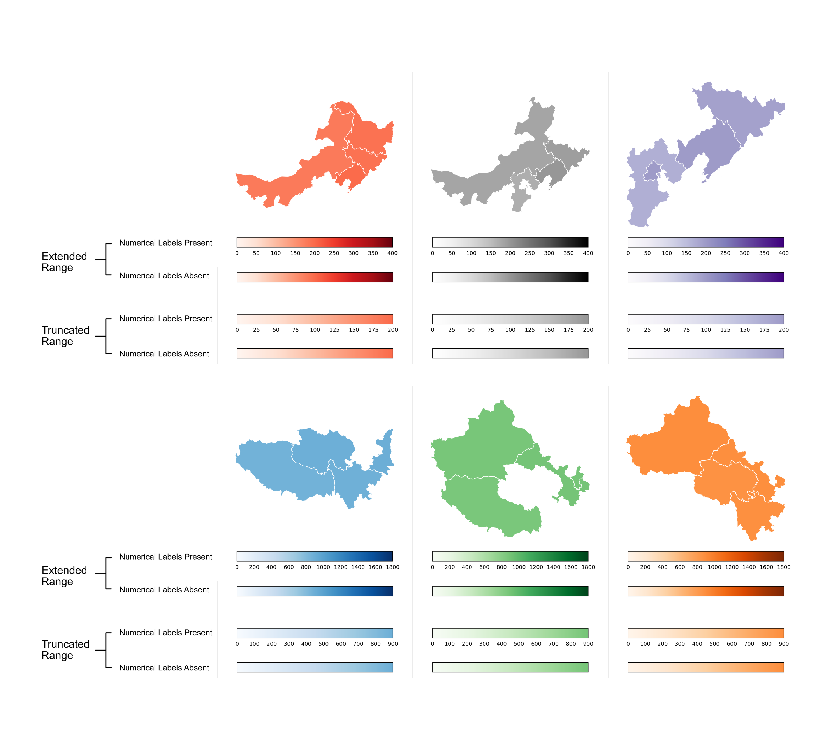
\includegraphics{ChoroplethMagnitude_files/figure-pdf/fig-example-stimuli-1.pdf}

}

\caption{\label{fig-example-stimuli}Example stimuli: six choropleth maps
showing fictitious pollution data. Four color legends are displayed
below each map, but only one color legend accompanied the map in each
trial. Color legends with extended ranges have a maximum value equal to
double the maximum plotted value (top row: 400; bottom row: 1800). Color
legends with truncated ranges have a maximum value equal to the maximum
plotted value in the map (top row: 200; bottom row: 900). During the
experiment, all six color scales were used in conjunction with all
maximum values.}

\end{figure}

\hypertarget{participants}{%
\subsection{Participants}\label{participants}}

We recruited participants using prolific.co. The experiment was
advertised to users with English language fluency, normal or
corrected-to-normal vision, and no experience of color deficiency, who
had previously participated in more than 100 studies on Prolific.
Participants were paid £3.50. Ethical approval was granted by our The
University of Manchester's Division of Neuroscience and Experimental
Psychology Ethics Committee (Ref. 2022-11115-23778).

In our pre-registration, we planned to exclude participants who failed
more than one attention check question, in order to exclude those who
were not sufficiently engaged in the task. However, when many more
participants than expected failed more than one attention check
question, this criteria was deemed too stringent and we instead awarded
payment to all participants who returned data, regardless of their
responses to attention check questions. Consequently, due to practical
constraints, we were unable to obtain a sample which met our
originally-specified sample size (N = 160) and our pre-registered
inclusion criteria. Therefore, we terminated data collection once the
sample of those who satisfied the attention check criteria was balanced
across all four Latin-squaring lists (N = 100; 25 participants per
list). We used this sample for our main analysis. As a compromise for
the reduction in experimental power, we also demonstrate below that the
pattern of effects is largely the same when analyzing the entire dataset
(those who satisfied attention check criteria and those who did not; N =
165). In Section 5, we discuss a possible reason for the
higher-than-expected rate of incorrect responses to attention check
questions. Demographic information is shown in
Table~\ref{tbl-demographics}.

\hypertarget{tbl-demographics}{}
\begin{table}
\caption{\label{tbl-demographics}Demographic Information }\tabularnewline

\centering\begingroup\fontsize{8}{10}\selectfont

\begin{tabular}{lrrrrrrrr}
\toprule
\multicolumn{1}{c}{ } & \multicolumn{3}{c}{Gender} & \multicolumn{2}{c}{Age} & \multicolumn{2}{c}{Graph Literacy} & \multicolumn{1}{c}{Education} \\
\cmidrule(l{3pt}r{3pt}){2-4} \cmidrule(l{3pt}r{3pt}){5-6} \cmidrule(l{3pt}r{3pt}){7-8} \cmidrule(l{3pt}r{3pt}){9-9}
Sample & Male (\%) & Female (\%) & Prefer not to say (\%) & Mean & SD & Mean & SD & High School
or Above (\%)\\
\midrule
N = 100 & 59.0 & 40.0 & 1.0 & 30.8 & 8.8 & 21.6 & 4.5 & 98.0\\
N = 165 & 53.9 & 45.5 & 0.6 & 31.8 & 10.1 & 21.8 & 4.5 & 98.8\\
\bottomrule
\end{tabular}
\endgroup{}
\end{table}

\hypertarget{procedure}{%
\subsection{Procedure}\label{procedure}}

The experiment was programmed using PsychoPy (Peirce \emph{et al.} 2019,
version 2022.1.4) and hosted on pavlovia.org. A link to an interactive
version of this experiment has been excluded from this manuscript for
anonymization purposes. Participants were instructed to use laptop or
desktop computers, rather than another type of device and were told that
the experiment was about using information to make decisions.
Participants were informed that in each map, each region's color
reflected its pollution level, and that data on different types of
pollution were shown throughout the experiment, with pollution levels
presented using standardized units.

In every experimental trial, the text above the map read `\emph{This map
shows the levels of a certain type of pollution, in four regions}'.
Participants were advised to read the question, which was presented
below the map: `\emph{How urgently should pollution levels in these
regions be addressed?}' This question was used in all experimental
trials, where the left anchor on the visual analogue response scale was
labeled `\emph{Not very urgently}' and the right anchor was labeled
`\emph{Very urgently}'. The instructions stated that higher pollution
levels need to be addressed more urgently than lower pollution levels.
Participants were permitted to move the response scale marker as many
times as they wished before continuing to the next trial.

Attention check items resembled normal trials except for the text
displayed. Participants were asked to move the marker to one of three
locations: `to the middle of the scale', `all the way to the \emph{'Not
very urgently'} end of the scale' or `all the way to the \emph{'Very
urgently'} end of the scale'. In experimental trials, response scale
granularity was set to 0, which permitted participants to place the
marker at any location along the response scale. In attention check
trials, response scale granularity was set to 0.5, so participants were
only permitted to place the marker at one of three locations specified
in the question: the leftmost point, the center of the scale, or the
rightmost point.

Following the final trial, participants were informed that both the data
presented, and the standardized units used, were fictitious. Finally,
participants were presented with a text box and the prompt `\emph{What
strategies did you use during the study? Do you have any comments about
the study? (optional)}'. Average completion time was 13.57 minutes (SD =
6.24 minutes) for those who satisfied the pre-registered attention check
criteria and 12.56 minutes (SD = 6.20 minutes) for the full sample.

\hypertarget{materials}{%
\subsection{Materials}\label{materials}}

Materials were generated using Python (version 3.9.12). Matplotlib
(version 3.5.1) was used to generate color legends and geoplot (version
0.5.1) was used for plotting geospatial data.

Each visualization contained a unique combination of four neighboring
Chinese provinces (except the six attention check items, which employed
six existing combinations used in the experimental items). China was
chosen to reduce the potential impact of prior knowledge, as Prolific's
participants tend to be located outside China. However, the choice of
country was not disclosed to participants and regions were not labeled.
The pollution data used were entirely fictitious, as were the
`standardized units' used to present the data.

The maximum value in the plotted data ranged from 200 to 900 (in
multiples of 100), and the values for the other three provinces were
between 10 and 30 units below this maximum value. Six Matplotlib color
scales (`Reds', `Greys', `Purples', `Blues', `Greens', `Oranges') were
each used once per maximum value. For each item, a `mappable' object
defined the mapping between numerical values and colors for both
truncated and extended color legends. The lightest color in the scale
was mapped to zero and the darkest color to double the maximum value.
This range was employed in the extended color legend. The truncated
color legend, on the other hand, terminated at the maximum value in the
data, so the range was halved (but the mapping between numerical values
and colors was retained). Where numerical labels were present, an
identical number of labels (between six and ten) appeared on both
versions of a color legend. Tick marks were absent from all color
legends.

\hypertarget{analysis}{%
\section{Analysis}\label{analysis}}

\hypertarget{analysis-methods}{%
\subsection{Analysis Methods}\label{analysis-methods}}

Analysis was conducted in R (R Core Team 2022, version 4.2.1).

Linear mixed-effects models were constructed using lme4 (Bates \emph{et
al.} 2015, version 1.1.31). Random effects structures were determined
using buildmer (Voeten 2022, version 2.7), which after identifying the
most complex random effects structure that could successfully converge
(see Barr \emph{et al.} 2013), then removed random effects terms which
did not significantly contribute towards explaining variance. In a
diversion from the pre-registered analysis plan, we excluded the
interaction term from the models used to test the main effects of color
legend range and numerical label presence.

\hypertarget{part-1-participants-satisfying-attention-check-criteria-n-100}{%
\subsection{Part 1: Participants Satisfying Attention Check Criteria (N
=
100)}\label{part-1-participants-satisfying-attention-check-criteria-n-100}}

\hypertarget{color-legend-ranges-and-numerical-labels}{%
\subsubsection{Color Legend Ranges and Numerical
Labels}\label{color-legend-ranges-and-numerical-labels}}

Figure~\ref{fig-main-effect-chart} shows the distribution of responses
for color legends with truncated and extended ranges.

\begin{figure}

{\centering 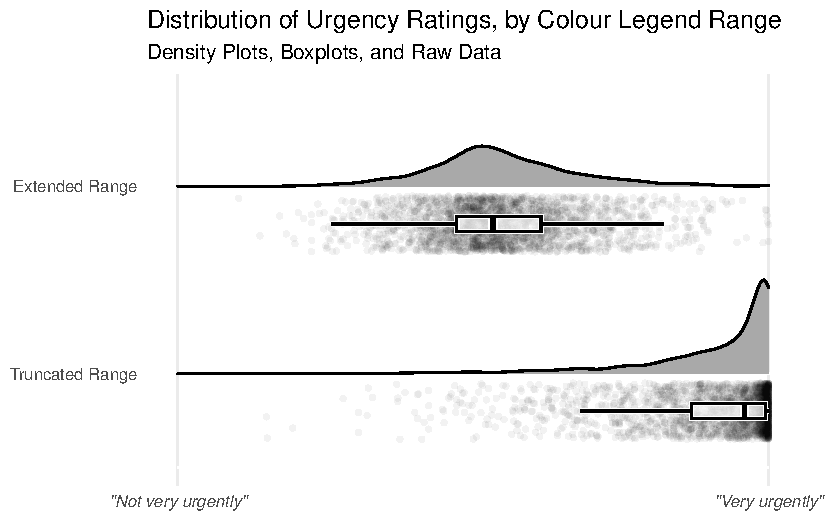
\includegraphics{ChoroplethMagnitude_files/figure-pdf/fig-main-effect-chart-1.pdf}

}

\caption{\label{fig-main-effect-chart}Visual analogue scale responses to
the question \emph{``How urgently should pollution levels in these
regions be addressed?''}. Distributions for the two conditions are shown
using histograms, boxplots, and raw data points representing individual
observations. In the `Extended Range' condition, the color legend's
upper bound was equal to double the maximum plotted value. In the
`Truncated Range' condition, the color legend's upper bound was equal to
the maximum plotted value.}

\end{figure}

Linear mixed-effects modelling revealed that urgency was rated as
significantly higher when the color legend had a truncated range (its
upper bound was equal to the maximum value in the dataset) compared to
when the color legend had an extended range (its upper bound was equal
to double the maximum value): \(\chi^2\)(1) = 225.41, p \textless{}
.001, \(\eta_p^2\) = 0.90.

Ratings were not significantly different when numerical labels were
present, compared to when they were absent: \(\chi^2\)(1) = 0.35, p =
.556, \(\eta_p^2\) \textless{} 0.01.

There was no interaction between color legend range and numerical
labels: \(\chi^2\)(1) = 1.73, p = .189, \(\eta_p^2\) = 0.02. These
models all employed random intercepts for participants with random
slopes for color legend range, numerical label presence, and the
interaction between these terms, plus random intercepts for items.

\hypertarget{data-visualization-literacy}{%
\subsubsection{Data Visualization
Literacy}\label{data-visualization-literacy}}

Adding participants' data visualization literacy as an additional fixed
effect did not remove the significant effect of color legend range:
\(\chi^2\)(1) = 260.93, p \textless{} .001, \(\eta_p^2\) = 0.89. This
indicates that differences in data visualization literacy cannot explain
this effect. The numerical label manipulation remained non-significant
when accounting for literacy (\(\chi^2\)(1) = 0.30, p = .586,
\(\eta_p^2\) \textless{} 0.01). The interaction remained non-significant
when accounting for literacy (\(\chi^2\)(1) = 3.21, p = .073,
\(\eta_p^2\) \textless{} 0.01). These models employed random intercepts
for participants with random slopes for color legend range and numerical
label presence, plus random intercepts for items with random slopes for
color legend range.

\hypertarget{part-2-all-participants-n-165}{%
\subsection{Part 2: All Participants (N =
165)}\label{part-2-all-participants-n-165}}

\hypertarget{color-legend-ranges-and-numerical-labels-1}{%
\subsubsection{Color Legend Ranges and Numerical
Labels}\label{color-legend-ranges-and-numerical-labels-1}}

The above analysis was conducted using data from the 100 participants
who satisfied the pre-registered attention check criteria. However,
smaller samples are associated with lower statistical power. Below, we
conduct the same analysis on the full sample of 165 participants (those
who satisfied the pre-registered attention check criteria and those who
did not).

Urgency was rated as significantly higher when a truncated color legend
range was used, compared to when an extended color legend range was
used: \(\chi^2\)(1) = 272.40, p \textless{} .001, \(\eta_p^2\) = 0.87.
Ratings were not significantly different when numerical labels were
present, compared to when they were absent: \(\chi^2\)(1) = 1.95, p =
.163, \(\eta_p^2\) = 0.01. These models employed random intercepts for
participants with random slopes for color legend range, numerical label
presence, and the interaction between these terms, plus random
intercepts for items with random slopes for color legend range.

There was a significant interaction between color legend range and
numerical label presence: \(\chi^2\)(1) = 6.41, p = .011, \(\eta_p^2\)
\textless{} 0.01. This model employed random intercepts for participants
with random slopes for color legend range and numerical label presence,
plus random intercepts for items with random slopes for color legend
range. We conducted pairwise comparisons with Sidak adjustment using the
emmeans package (Lenth 2021). For choropleth maps with extended color
legend ranges, there was no difference between ratings for labeled and
unlabeled color legends: z = 0.59, p = .962, Cohen's \emph{d} = 0.02.
For choropleth maps with truncated color legend ranges, higher ratings
were awarded when numerical labels were absent, compared to when they
were present: z = 2.99, p = .011, Cohen's \emph{d} = 0.10.
Figure~\ref{fig-interaction-chart} displays the means and 95\%
confidence intervals for each combination of conditions, for both
samples of participants: those who satisfied the pre-registered
attention check criteria, and the full sample.

\begin{figure}

{\centering 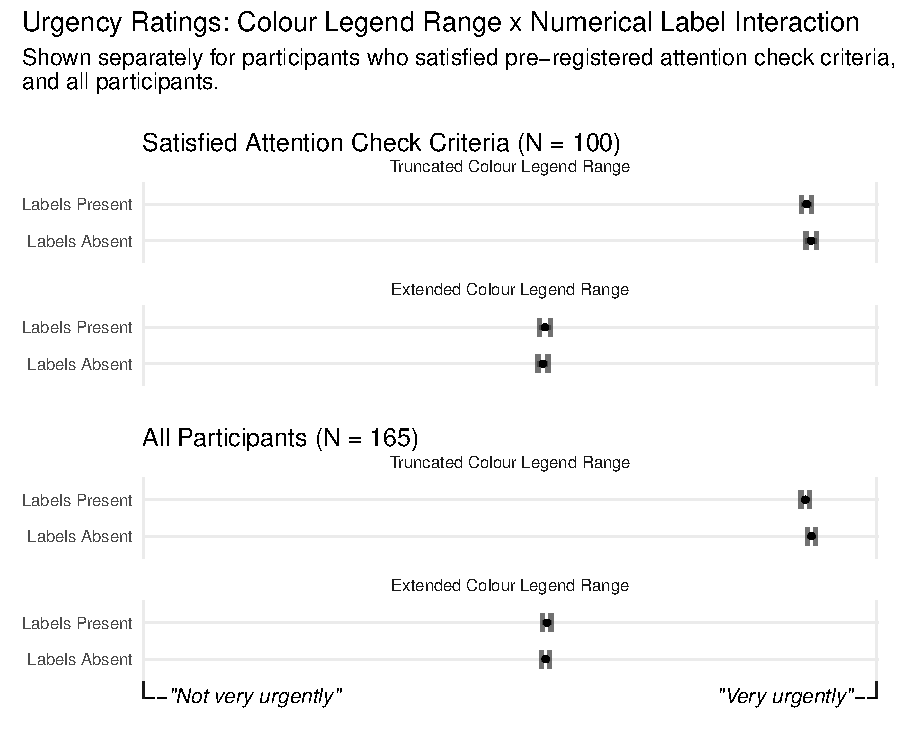
\includegraphics{ChoroplethMagnitude_files/figure-pdf/fig-interaction-chart-1.pdf}

}

\caption{\label{fig-interaction-chart}Mean urgency ratings showing the
interaction between color legend range and numerical label presence,
displayed separately for the different samples of participants. Error
bars show 95\% confidence intervals around the means.}

\end{figure}

\hypertarget{data-visualization-literacy-1}{%
\subsubsection{Data Visualization
Literacy}\label{data-visualization-literacy-1}}

The same pattern of results was observed when accounting for differences
in data visualization literacy. There was a significant effect of color
legend range (\(\chi^2\)(1) = 272.45, p \textless{} .001, \(\eta_p^2\) =
0.87) and no effect of numerical label presence (\(\chi^2\)(1) = 2.09, p
= .148), \(\eta_p^2\) = 0.01. The interaction between color legend range
and numerical label presence remained: \(\chi^2\)(1) = 6.47, p = .011,
\(\eta_p^2\) \textless{} 0.01. These models employed random intercepts
for participants with random slopes for color legend range and numerical
label presence, plus random intercepts for items with random slopes for
color legend range.

\hypertarget{exploratory-analysis}{%
\subsection{Exploratory Analysis}\label{exploratory-analysis}}

Our pre-registered analysis did not detect an effect of the presence of
numerical values on urgency ratings. However, a more fine-grained
analysis can explore the role of numerical labels with greater
sensitivity. This exploratory analysis examines whether urgency ratings
are influenced by the actual numerical values displayed. We
systematically varied the maximum value displayed in each map, which
ranged from 200 to 900. Other plotted values were defined in relation to
this value: between 10 and 30 units less than the maximum value.
Modelling the effect of different maximum values on ratings will reveal
whether judgments were informed by the numerical values displayed.

When considering only maps with numerical labels present, ratings
increased as a function of maximum value (\(\chi^2\)(1) = 27.90, p
\textless{} .001, \(\eta_p^2\) = 0.48). This model employed random
intercepts for participants with random slopes for color legend range,
plus random intercepts for items with random slopes for color legend
range. However, ratings also increased as a function of maximum value
even when numerical labels were absent (\(\chi^2\)(1) = 16.85, p
\textless{} .001, \(\eta_p^2\) = 0.32). This model employed random
intercepts for participants with random slopes for color legend range,
plus random intercepts for items. There was no significant interaction
between maximum value and numerical label presence (\(\chi^2\)(1) =
2.22, p = .137, \(\eta_p^2\) \textless{} 0.01). This model employed
random intercepts for participants with random slopes for color legend
range and numerical label presence, plus random intercepts for items
with random slopes for color legend range.

This suggests that the numerical labels themselves were not responsible
for the effect of maximum value. Instead, this effect may have been
driven by the appearance of the choropleth map. The color for the
maximum value was identical in each map with the same color palette, but
the three \emph{accompanying} values in each map were always between 10
and 30 units less than the maximum value. Consequently, these values
were represented by darker colors when the maximum value was higher,
thus conveying greater overall magnitude. Color legend range
(\(\eta_p^2\) = 0.89) remains a greater influence than maximum value
(\(\eta_p^2\) = 0.44).

In the models for participants who satisfied the pre-registered
attention check criteria \emph{and} those who did not (N = 165), there
were significant effects of maximum value, for both maps with labeled
color legends (\(\chi^2\)(1) = 28.55, p \textless{} .001, \(\eta_p^2\) =
0.50) and also maps with unlabeled color legends (\(\chi^2\)(1) = 16.27,
p \textless{} .001, \(\eta_p^2\) = 0.32). These models employed random
intercepts for participants with random slopes for color legend range,
plus random intercepts for items with random slopes for color legend
range. There was no significant interaction between maximum value and
numerical label presence (\(\chi^2\)(1) = 3.51, p = .061, \(\eta_p^2\)
\textless{} 0.01). This model employed random intercepts for
participants with random slopes for color legend range and numerical
label presence, plus random intercepts for items with random slopes for
color legend range. Color legend range (\(\eta_p^2\) = 0.87) remains a
greater influence than maximum value (\(\eta_p^2\) = 0.45).

\hypertarget{discussion}{%
\section{Discussion}\label{discussion}}

Choropleth maps are typically used to convey spatial variability, but
may alternatively be employed to convey overall magnitude. This
experiment clearly demonstrated that the range of the accompanying color
legend influences interpretations of magnitude in such choropleth maps.
When the color legend's upper bound was equivalent to the maximum
plotted value, participants rated the urgency of addressing pollution
levels as higher, compared to when the color legend's upper bound was
equal to double the maximum plotted value. This illustrates that viewers
use color legends to put numbers' magnitudes into perspective,
interpreting magnitude with respect to the range of the color legend. A
color legend does not only provide a mapping between numerical values
and colors, it also provides a range of values relevant for considering
the magnitude of presented data.

Crucially, the colors used to display the data in the maps, as well as
the underlying numerical values, were identical across conditions.
Therefore, differences in participants' judgments between conditions
were not due to these factors. Instead, participants formed different
impressions of these data based on the context in which they were
presented. We do not suggest that one color legend arrangement used in
this experiment was misleading and the other truthful. Rather, we
suggest that, under certain circumstances, either could be characterized
as misleading. Thus, doctored data and deliberate deception are not the
only practices behind problematic visualizations.

Color legends simultaneously encode changes in number through both color
and physical position. Different values are represented by different
colors \emph{and} occupy different positions on the color legend. In the
present experiment, plotted values' analogous positions in the truncated
color legend were on the far right hand side, and their corresponding
colors were among the darkest in the legend. On the other hand, plotted
values' analogous positions were in the middle of the extended color
legend, and their corresponding colors were neither the darkest nor the
lightest in the legend. This experiment cannot determine whether the
location of plotted values on the legend, the range of colors included
in the legend, or both of these factors, influenced processing of
magnitude. The manipulation of numerical labels does not assist in
answering this question because color legends still encode changes in
number even when these changes are not labeled. However, this question
may have little practical relevance since these aspects are
intrinsically linked in a typical color legend.

In this experiment, the width of truncated and extended color legends
was identical. In the truncated color legend, a smaller range of colors
spanned the same distance: there was less variation in color over the
same amount of space. We have not identified any way in which this could
explain the present set of results.

\hypertarget{additional-analyses}{%
\subsection{Additional Analyses}\label{additional-analyses}}

Accounting for subjective data visualization literacy did not change the
pattern of results. This suggests that data visualization literacy is
not responsible for the observed effect of color legend range on
interpretations of magnitude. This accords with the finding that data
visualization literacy levels did not explain the bias in judgments
caused by truncated axes (Yang \emph{et al.} 2021). Yang \emph{et al.}
(2021) suggest that data visualization literacy measures capture whether
an individual has the skills required for comprehending typical chart
formats. However, they do not appear to extend to aspects of
visualization comprehension which are informed by intuitive judgments
rather than basic training.

Our results demonstrate that numerical labels did not influence
judgments. Our pre-registered analysis found that there was no
difference between ratings for maps with and without numerical labels on
the color legend. An exploratory analysis examining this further also
indicates that increases in the numerical values displayed on the color
legend were not responsible for greater urgency ratings. Instead, it is
likely that increased urgency ratings associated with higher maximum
values were related to the presence of darker colors in the maps. This
was a consequence of accompanying data points' increased proximity to
the maximum value at higher maximum values (see
Figure~\ref{fig-example-stimuli}).

For data quality reasons, we conducted our main analysis on a sample of
100 participants who met our pre-registered attention check threshold
(no more than one of six attention check questions answered
incorrectly). However, we also conducted the same analysis on the full
sample of 165 participants, in the interest of validity. The pattern of
results in the two samples was extremely similar, indicating similar
levels of engagement with the task regardless of attention check scores.
Participants may have withdrawn attention from the accompanying text and
question once they were aware that these did not change across
experimental trials, consequently failing to notice attention-check
trials.

The only difference between the pattern of results for these two samples
was the interaction between color legend range and numerical label
presence. This interaction was not observed in the more selective sample
but observed in the full sample. However,
Figure~\ref{fig-interaction-chart} illustrates that the pattern of
responses was remarkably similar. In both samples, the difference
between ratings for the labeled and unlabeled versions of the truncated
color legend was very small, which suggests the significant result was
driven by low variance within conditions and increased statistical power
in the larger sample. The inconsistency in inferential statistics
between samples suggests that this interaction, if not spurious, is not
particularly robust.

\hypertarget{relationship-to-prior-work}{%
\subsection{Relationship to Prior
Work}\label{relationship-to-prior-work}}

Investigations into chart design have revealed that the range of values
surrounding plotted data influences interpretations. Several experiments
have observed that participants use axes as a source of context for
assessing the magnitude of difference between values (Pandey \emph{et
al.} 2015, Witt 2019, Correll \emph{et al.} 2020, Yang \emph{et al.}
2021). The present experiment provides further evidence for a
less-frequently explored phenomenon: that design choices can affect
judgments of \emph{the magnitude of values themselves}. Like Stone
\emph{et al.} (2003) and Sandman \emph{et al.} (1994), we demonstrate
that plotted values seem greater when they are closer to a data
visualization's upper bound. However, this experiment also demonstrates
that these types of effects are not unique to data visualizations using
geometric encodings. Choropleth maps, where the range of values is
presented in a color legend, can also elicit this bias. Arguably, the
manipulation in choropleth maps is even more subtle, because of the
unique way that choropleth maps separate encoded data from the color
legend. In data visualizations such as bar charts, changing the range of
values alters the appearance of the data itself (an extended y-axis
results in a compressed bar). The present experiment's findings are
particularly striking given that the appearance of data remained
consistent despite changes to the color legend's upper bound. This
suggests differences in judgments were not driven by the visual
appearance of the data, but by the interpretation of the data in
relation to the range of values in the color legend.

This finding is also connected to research on the interpretation of
quantity in colormap visualizations. Schiewe (2019) observed that
assessment of values presented in choropleths are driven by the coverage
of darker colors. We expand upon this work by identifying another factor
which biases judgments of data in choropleth maps, yet does not change
the appearance of the map itself. Like Correll \emph{et al.} (2018), we
demonstrate that manipulating a color legend is sufficient to influence
participants' responses. Schloss et al.'s (2019) results demonstrated
that a colormap's background color is interpreted as corresponding to
the smallest quantity when a scale appears to vary in opacity. That is,
background color provides a cue to the size of data points when taken to
represent the minimum value. The present experiment demonstrates that,
like quantity judgments, magnitude judgments are also driven by visual
cues to the minimum and maximum values.

A bias wherein the same values are judged differently depending on their
surrounding context is often described as a framing effect (Tversky and
Kahneman 1974). This bias involves using inessential accompanying
information to inform one's judgement, rather than discounting this
information in order to generate a wholly disinterested assessment.
Other research has also demonstrated that the interpretation of
numerical values depends on their placement within a range. For example,
the same salary is rated as more desirable when it appears near the top
rather than the bottom of a range (Brown \emph{et al.} 2008). The
present experiment translates this effect to the visual domain. As Yang
\emph{et al.} (2021) suggest, biases in viewers' processing of
information in data visualizations can be explained with reference to
Grice's (1975) cooperative principle. Applied to the present experiment,
this suggests that viewers would interpret the implication of certain
magnitudes through the color legend design as indicative of the
designer's intention to communicate values' true magnitudes.

\hypertarget{limitations-and-future-research-directions}{%
\subsection{Limitations and Future Research
Directions}\label{limitations-and-future-research-directions}}

Choropleth maps are typically designed to communicate differences
between values, rather than values' magnitudes. Discrimination between
values is facilitated when the color legend's bounds are equal to the
minimum and maximum values in the dataset. Therefore, designers may have
to make a trade-off between conveying magnitude and conveying
differences. Which aspect of the data a designer wishes to emphasize
will depend on the purpose of their data visualization. For example, a
designer may wish to highlight the geographical differences in the
construction of new houses, or may wish to highlight the fact that there
is no region where targets are being met. The work reported here
suggests that extending the range of the color legend beyond the range
of the observed data would promote the latter message.

It is important to recognize that a color scale's bounds may not always
be interpreted as a complete and accurate source of context for
assessing magnitude. Pollution measurements are likely not among the
most intuitive numbers to interpret, and in the present experiment, even
viewers well-versed in pollution data were prohibited from applying
their knowledge, since the fictitious data were presented using
fictitious units. The influence of existing knowledge was eliminated to
facilitate examination of the cognitive mechanism involved in magnitude
judgments. Therefore, in this experiment, there were no \emph{external}
cues to magnitude. Consequently, our findings are most relevant for
understanding interpretation of magnitude where units are unfamiliar or
insignificant. Familiarity with a data visualization's subject matter
will typically provide an ability to independently assess magnitudes
based on presented values only, which may reduce the influence of design
choices. In addition, certain forms of number may carry cues to
magnitude even in the absence of existing knowledge. For example, when
assessing certain proportions, viewers are likely to be aware that 100\%
is the maximum possible value and 0\% the minimum. Future work should
explore the degree to which these scenarios affect how color legends
inform magnitude judgments.

Future work should quantify the difference between different color
legend ranges in concrete units (e.g., a specific difference in
financial investment, or a specific time-frame for resolving an issue).
The visual analogue scale used in our investigation does not permit
this. However, it was able to reveal that interpretations of magnitude
differed between conditions, reflecting the type of inferences that are
likely to precede decision-making. The within-participants design
ensures that participants' different notions of urgency do not interfere
with comparisons between experimental conditions. Future work should
also examine a wider variety of topics beyond pollution data in order to
examine generalizability. However, our investigation has nonetheless
produced informative results, and the observed bias, a framing effect,
occurs widely.

Numerical labels at the extremes of color legends are sometimes
open-ended. That is, a label at the lower bound may be `\textless30'
rather than `30'. This interrupts the one-to-one mapping between colors
and values. Instead, a specific position and color on the color legend
may represent multiple corresponding numerical values. Consequently,
\emph{more extreme} values may exist in the data than those represented
by the extremes of the legend. This introduces ambiguity regarding the
relevant range of values to consider when assessing magnitude, making
the color legend a less informative reference. Future research should
examine whether the present findings are replicated when a color legend
uses this type of numerical label at its extremes, or whether viewers
treat color legends with these labels as a weaker cue to plotted values'
magnitudes.

\hypertarget{implications}{%
\subsection{Implications}\label{implications}}

The present experiment contributes to our understanding of cognitive
mechanisms involved in assessing magnitudes in choropleth maps. We
observed that assessments are informed by the range of the color legend,
demonstrating that color legends can be exploited to influence viewers'
judgments of data points' magnitudes. Further work is required in order
to identify various factors influencing the strength of this effect, but
the essential implication entails designers considering how magnitude
appears as a result of their chosen color legend's range. Without
deliberate consideration about the choice of value for a color legend's
upper bound, misleading visualizations may emerge. However, like Correll
\emph{et al.} (2020), we argue there can be no \emph{a priori} system
for identifying a range of values that guarantees an unbiased
visualization. Instead, the range of the color legend should be
appropriate for the data displayed, the intended message, and the task.
There are also implications for data visualization software developers
in facilitating designers' ability to specify a custom color legend
range when required.

\hypertarget{conclusion}{%
\section{Conclusion}\label{conclusion}}

Understanding the consequences of design choices is crucial for
understanding how to present data effectively. In choropleth maps, the
upper bound of the accompanying color legend influences how large or
small plotted values appear to viewers. Data points' proximity to the
upper bound increases impressions of their magnitude. This finding
provides insight into the processing of choropleth maps designed to
convey overall magnitude, and promotes use of a suitable range of values
on a color legend.

\hypertarget{acknowledgements}{%
\section*{Acknowledgements}\label{acknowledgements}}
\addcontentsline{toc}{section}{Acknowledgements}

This work was supported by the Economic and Social Research Council
under Grant ES/P000665/1.

\hypertarget{disclosure-statement}{%
\section*{Disclosure Statement}\label{disclosure-statement}}
\addcontentsline{toc}{section}{Disclosure Statement}

The authors report there are no competing interests to declare.

\newpage{}

\hypertarget{references}{%
\section*{References}\label{references}}
\addcontentsline{toc}{section}{References}

\hypertarget{refs}{}
\begin{CSLReferences}{1}{0}
\leavevmode\vadjust pre{\hypertarget{ref-barr_random_2013}{}}%
Barr, D.J., Levy, R., Scheepers, C., and Tily, H.J., 2013.
\href{https://doi.org/10.1016/j.jml.2012.11.001}{Random effects
structure for confirmatory hypothesis testing: {Keep} it maximal}.
\emph{Journal of Memory and Language}, 68 (3), 255--278.

\leavevmode\vadjust pre{\hypertarget{ref-bates_fitting_2015}{}}%
Bates, D., Mächler, M., Bolker, B., and Walker, S., 2015.
\href{https://doi.org/10.18637/jss.v067.i01}{Fitting {Linear}
{Mixed}-{Effects} {Models} {Using} \textbf{lme4}}. \emph{Journal of
Statistical Software}, 67 (1).

\leavevmode\vadjust pre{\hypertarget{ref-brown_does_2008}{}}%
Brown, G.D.A., Gardner, J., Oswald, A.J., and Qian, J., 2008.
\href{https://doi.org/10.1111/j.1468-232X.2008.00525.x}{Does {Wage}
{Rank} {Affect} {Employees}' {Well}-being?} \emph{Industrial Relations},
47 (3), 355--389.

\leavevmode\vadjust pre{\hypertarget{ref-correll_truncating_2020}{}}%
Correll, M., Bertini, E., and Franconeri, S., 2020.
\href{https://doi.org/10.1145/3313831.3376222}{Truncating the
{Y}-{Axis}: {Threat} or {Menace}?} \emph{In}: \emph{Proceedings of the
2020 {CHI} {Conference} on {Human} {Factors} in {Computing} {Systems}}.
Honolulu HI USA: ACM, 1--12.

\leavevmode\vadjust pre{\hypertarget{ref-correll_value-suppressing_2018}{}}%
Correll, M., Moritz, D., and Heer, J., 2018.
\href{https://doi.org/10.1145/3173574.3174216}{Value-{Suppressing}
{Uncertainty} {Palettes}}. \emph{In}: \emph{Proceedings of the 2018
{CHI} {Conference} on {Human} {Factors} in {Computing} {Systems}}.
Montreal QC Canada: ACM, 1--11.

\leavevmode\vadjust pre{\hypertarget{ref-dasgupta_effect_2020}{}}%
Dasgupta, A., Poco, J., Rogowitz, B., Han, K., Bertini, E., and Silva,
C.T., 2020. \href{https://doi.org/10.1109/TVCG.2018.2876539}{The
{Effect} of {Color} {Scales} on {Climate} {Scientists}' {Objective} and
{Subjective} {Performance} in {Spatial} {Data} {Analysis} {Tasks}}.
\emph{IEEE Transactions on Visualization and Computer Graphics}, 26 (3),
1577--1591.

\leavevmode\vadjust pre{\hypertarget{ref-driessen_misleading_2022}{}}%
Driessen, J.E.P., Vos, D.A.C., Smeets, I., and Albers, C.J., 2022.
\href{https://doi.org/10.1371/journal.pone.0265823}{Misleading graphs in
context: {Less} misleading than expected}. \emph{PLOS ONE}, 17 (6),
e0265823.

\leavevmode\vadjust pre{\hypertarget{ref-fischer_federal_2021}{}}%
Fischer, J. and Ali, A., 2021.
\href{https://www.dataforprogress.org/blog/2021/12/10/a-federal-ban-on-abortion-is-wildly-unpopular-in-all-50-states}{A
{Federal} {Ban} on {Abortion} is {Wildly} {Unpopular} in {All} 50
{States}}. \emph{Data For Progress}.

\leavevmode\vadjust pre{\hypertarget{ref-galesic_graph_2011}{}}%
Galesic, M. and Garcia-Retamero, R., 2011.
\href{https://doi.org/10.1177/0272989X10373805}{Graph {Literacy}: {A}
{Cross}-{Cultural} {Comparison}}. \emph{Medical Decision Making}, 31
(3), 444--457.

\leavevmode\vadjust pre{\hypertarget{ref-garcia-retamero_measuring_2016}{}}%
Garcia-Retamero, R., Cokely, E.T., Ghazal, S., and Joeris, A., 2016.
\href{https://doi.org/10.1177/0272989X16655334}{Measuring {Graph}
{Literacy} without a {Test}: {A} {Brief} {Subjective} {Assessment}}.
\emph{Medical Decision Making}, 36 (7), 854--867.

\leavevmode\vadjust pre{\hypertarget{ref-garcia-retamero_who_2010}{}}%
Garcia-Retamero, R. and Galesic, M., 2010.
\href{https://doi.org/10.1016/j.socscimed.2009.11.031}{Who proficts from
visual aids: {Overcoming} challenges in people's understanding of
risks}. \emph{Social Science \& Medicine}, 70 (7), 1019--1025.

\leavevmode\vadjust pre{\hypertarget{ref-grice_logic_1975}{}}%
Grice, P., 1975. Logic and {Conversation}. \emph{In}: P. Cole and J.L.
Morgan, eds. \emph{Syntax and {Semantics} {Vol}.3: {Speech} {Acts}}. New
York: Academic Press, 41--58.

\leavevmode\vadjust pre{\hypertarget{ref-harrower_colorbrewerorg_2003}{}}%
Harrower, M. and Brewer, C.A., 2003.
\href{https://doi.org/10.1179/000870403235002042}{{ColorBrewer}.org:
{An} {Online} {Tool} for {Selecting} {Colour} {Schemes} for {Maps}}.
\emph{The Cartographic Journal}, 40 (1), 27--37.

\leavevmode\vadjust pre{\hypertarget{ref-hu_foreground-background_2014}{}}%
Hu, T.-Y., Jiang, X.-W., Xie, X., Ma, X.-Q., and Xu, C., 2014.
Foreground-background salience effect in traffic risk communication.
\emph{Judgment and Decision Making}, 9 (1), 8.

\leavevmode\vadjust pre{\hypertarget{ref-hunter_matplotlib_2007}{}}%
Hunter, J.D., 2007.
\href{https://doi.org/10.1109/MCSE.2007.55}{Matplotlib: {A} {2D}
{Graphics} {Environment}}. \emph{Computing in Science \& Engineering}, 9
(3), 90--95.

\leavevmode\vadjust pre{\hypertarget{ref-lenth_emmeans_2021}{}}%
Lenth, R.V., 2021.
\href{https://CRAN.R-project.org/package=emmeans}{Emmeans: {Estimated}
{Marginal} {Means}, aka {Least}-{Squares} {Means}}.

\leavevmode\vadjust pre{\hypertarget{ref-lin_selecting_2013}{}}%
Lin, S., Fortuna, J., Kulkarni, C., Stone, M., and Heer, J., 2013.
\href{https://doi.org/10.1111/cgf.12127}{Selecting
{Semantically}-{Resonant} {Colors} for {Data} {Visualization}}.
\emph{Computer Graphics Forum}, 32 (3pt4), 401--410.

\leavevmode\vadjust pre{\hypertarget{ref-okan_probability_2020}{}}%
Okan, Y., Stone, E.R., Parillo, J., Bruine de Bruin, W., and Parker,
A.M., 2020. \href{https://doi.org/10.1111/risa.13431}{Probability {Size}
{Matters}: {The} {Effect} of {Foreground}‐{Only} versus
{Foreground}+{Background} {Graphs} on {Risk} {Aversion} {Diminishes}
with {Larger} {Probabilities}}. \emph{Risk Analysis}, 40 (4), 771--788.

\leavevmode\vadjust pre{\hypertarget{ref-pandey_how_2015}{}}%
Pandey, A.V., Rall, K., Satterthwaite, M.L., Nov, O., and Bertini, E.,
2015. \href{https://doi.org/10.1145/2702123.2702608}{How {Deceptive} are
{Deceptive} {Visualizations}?: {An} {Empirical} {Analysis} of {Common}
{Distortion} {Techniques}}. \emph{In}: \emph{Proceedings of the 33rd
{Annual} {ACM} {Conference} on {Human} {Factors} in {Computing}
{Systems} - {CHI} '15}. Seoul, Republic of Korea: ACM Press, 1469--1478.

\leavevmode\vadjust pre{\hypertarget{ref-peirce_psychopy2_2019}{}}%
Peirce, J., Gray, J.R., Simpson, S., MacAskill, M., Höchenberger, R.,
Sogo, H., Kastman, E., and Lindeløv, J.K., 2019.
\href{https://doi.org/10.3758/s13428-018-01193-y}{{PsychoPy2}:
{Experiments} in behavior made easy}. \emph{Behavior Research Methods},
51 (1), 195--203.

\leavevmode\vadjust pre{\hypertarget{ref-r_core_team_r_2022}{}}%
R Core Team, 2022. \href{https://www.R-project.org/}{R: {A} {Language}
and {Environment} for {Statistical} {Computing}}.

\leavevmode\vadjust pre{\hypertarget{ref-sandman_high_1994}{}}%
Sandman, P.M., Weinstein, N.D., and Miller, P., 1994.
\href{https://doi.org/10.1111/j.1539-6924.1994.tb00026.x}{High {Risk} or
{Low}: {How} {Location} on a "{Risk} {Ladder}" {Affects} {Perceived}
{Risk}}. \emph{Risk Analysis}, 14 (1), 35--45.

\leavevmode\vadjust pre{\hypertarget{ref-schiewe_empirical_2019}{}}%
Schiewe, J., 2019.
\href{https://doi.org/10.1007/s42489-019-00026-y}{Empirical {Studies} on
the {Visual} {Perception} of {Spatial} {Patterns} in {Choropleth}
{Maps}}. \emph{KN - Journal of Cartography and Geographic Information},
69 (3), 217--228.

\leavevmode\vadjust pre{\hypertarget{ref-schloss_mapping_2019}{}}%
Schloss, K.B., Gramazio, C.C., Silverman, A.T., Parker, M.L., and Wang,
A.S., 2019. \href{https://doi.org/10.1109/TVCG.2018.2865147}{Mapping
{Color} to {Meaning} in {Colormap} {Data} {Visualizations}}. \emph{IEEE
Transactions on Visualization and Computer Graphics}, 25 (1), 810--819.

\leavevmode\vadjust pre{\hypertarget{ref-stone_foregroundbackground_2003}{}}%
Stone, E.R., Sieck, W.R., Bull, B.E., Frank Yates, J., Parks, S.C., and
Rush, C.J., 2003.
\href{https://doi.org/10.1016/S0749-5978(03)00003-7}{Foreground:background
salience: {Explaining} the effects of graphical displays on risk
avoidance}. \emph{Organizational Behavior and Human Decision Processes},
90 (1), 19--36.

\leavevmode\vadjust pre{\hypertarget{ref-stone_effects_1997}{}}%
Stone, E.R., Yates, J.F., and Parker, A.M., 1997.
\href{https://doi.org/10.1037/1076-898X.3.4.243}{Effects of numerical
and graphical displays on professed risk-taking behavior.} \emph{Journal
of Experimental Psychology: Applied}, 3 (4), 243--256.

\leavevmode\vadjust pre{\hypertarget{ref-stone_engineering_2014}{}}%
Stone, M., Szafir, D.A., and Setlur, V., 2014. An {Engineering} {Model}
for {Color} {Difference} as a {Function} of {Size}. Boston,
Massachusetts: Society for Imaging Science; Technology, 6.

\leavevmode\vadjust pre{\hypertarget{ref-szafir_adapting_2014}{}}%
Szafir, D.A., Stone, M., and Gleicher, M., 2014. Adapting {Color}
{Difference} for {Design}. Boston, Massachusetts: Society for Imaging
Science; Technology, 6.

\leavevmode\vadjust pre{\hypertarget{ref-taylor_misleading_1986}{}}%
Taylor, B.G. and Anderson, L.K., 1986. Misleading {Graphs}: {Guidelines}
for the {Accountant}. \emph{Journal of Accountancy}, 162 (4), 126--135.

\leavevmode\vadjust pre{\hypertarget{ref-tversky_judgment_1974}{}}%
Tversky, A. and Kahneman, D., 1974.
\href{https://doi.org/10.1126/science.185.4157.1124}{Judgment under
{Uncertainty}: {Heuristics} and {Biases}}. \emph{Science}, 185 (4157),
1124--1131.

\leavevmode\vadjust pre{\hypertarget{ref-voeten_buildmer_2022}{}}%
Voeten, C.C., 2022.
\href{https://CRAN.R-project.org/package=buildmer}{Buildmer: {Stepwise}
{Elimination} and {Term} {Reordering} for {Mixed}-{Effects}}.

\leavevmode\vadjust pre{\hypertarget{ref-wickham_ggplot2_2016}{}}%
Wickham, H., 2016. \emph{ggplot2}. New York, NY: Springer
Science+Business Media, LLC.

\leavevmode\vadjust pre{\hypertarget{ref-witt_graph_2019}{}}%
Witt, J.K., 2019. \href{https://doi.org/10.15626/MP.2018.895}{Graph
{Construction}: {An} {Empirical} {Investigation} on {Setting} the
{Range} of the {Y}-{Axis}}. \emph{Meta-Psychology}, 3.

\leavevmode\vadjust pre{\hypertarget{ref-yang_truncating_2021}{}}%
Yang, B.W., Vargas Restrepo, C., Stanley, M.L., and Marsh, E.J., 2021.
\href{https://doi.org/10.1016/j.jarmac.2020.10.002}{Truncating bar
graphs persistently misleads viewers.} \emph{Journal of Applied Research
in Memory and Cognition}, 10 (2), 298--311.

\end{CSLReferences}



\end{document}
